\chapter{Performance Analysis}\label{cap:rendimiento}
\noindent In this chapter qosh performance will be evaluated deployed over a real cluster. The execution environment will be described first and the metrics collected will be analyzed and put in context thereafter.

\section{Testing Environment}\label{sec:entornodeprueba}
\noindent Figure \ref{fig:clusterdespliegue} shows how the cluster is configured. The leftmost part of the figure shows the Cloud Controller; the rightmost, the Cloud Node. The Cloud Controller has been put through a full OpenStack Folsom installation --- except for Cinder, Swift or Quantum as they will not used ---, plus MySQL, Fabric and Qpid as message broker. In the Cloud Node only the bare minimum to support VM execution has been installed --- OpenStack Compute. The other required \emph{amenities} of the Cloud Node are delegated to the Controller via Qpid.

\begin{figure}[tbp]
\begin{center}
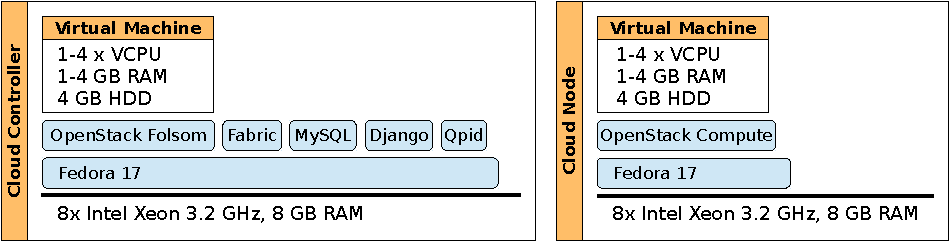
\includegraphics[width=0.99\textwidth]{imagenes/038.pdf}
 \caption{Deployment morphology}
\label{fig:clusterdespliegue}
\end{center}
\end{figure}

Regarding the physical layer, both nodes posses the same hardware configuration: Octa core Intel Xeon processor @ 3.2 \emph{GHz} with VT-x, 8 GB of RAM, 200 GB SATA 3 Gb/s 7200 RPM and Gigabit networking interface.

The Hadoop virtual image, whose creation procedure is described in section \ref{subsec:maquinavirtual}, will be used to create the VM instances that will effectively carry out the computations. Hadoop version is 1.0.4 and JRE's is 1.7v6 from Oracle. Figure \ref{fig:clusterdespliegue} shows the Hadoop VM in context. This instance will be increasingly provided from 1 to 4 GB of RAM and the same number of VCPUs to assess qosh's scaling. This varying amount of RAM will be shared between the guest OS and the JVM. The deployment has been configured to allow Hadoop to address all the memory in the VM --- except for those addresses in use by the OS and the JVM.

\section{Testing Methodology}\label{sec:metodologiaprueba}
\noindent This section contains both in and out scalability analysis and a study on the behavior on increasing input sizes. To evaluate how qosh scales, a map reduce work flow, large enough to stress every instance in the virtual cluster, will be fed to Hadoop; the work flow will count the words in 62.5 MB of plain text.

To actually assess the horizontal scalability, the size of the virtual cluster will progressively be doubled starting from one instance up to four. To test vertical scalability, two VMs will be initially spawned with 1 GB of RAM each, to have their RAM and VCPU count doubled on each test case until reaching 4 GB. Finally, to evaluate running time tendency input text size will be doubled from the original 62.5 MB to 250 MB.

As Glance and Compute cooperate to cache images, the time required to start an instance of some image will be longer the first time it launches, effectively skewing results. To get rid of those divergences, the instances on each flavor will be \textbf{warmed} by starting and destroying them before taking measures.

\emph{A priori}, the expected variance of the timings between executions is small enough to consider \emph{ten} to be a representative number of repeated measures --- this hypothesis will be validated \emph{a posteriori} on analyzing the results. To measure timings, the code will include a set of time marks that will help take apart the following times:

\begin{description}
    \item[Deploying:] time elapsed since the virtual cluster creation request is send until every instance is accessible.
    \item[Configuring:] time required to establish the Hadoop execution environment. It comprises the time to configure the virtual Hadoop cluster plus the time to distribute input data onto HDFS.
    \item[MapReducing:] time dedicated by Hadoop to execute the \emph{wordcount} work flow.
    \item[Cleaning:] time required to wipe out the execution environment. It does not include the time it takes OpenStack to completely remove the instances.
    \item[Total:] 
\end{description}

It should be noted that the timings shown are the averaged results of the ten executions in each case.

\section{Analysis of the Results}\label{sec:analisisresultados}

\begin{figure}[tbp]
\begin{center}
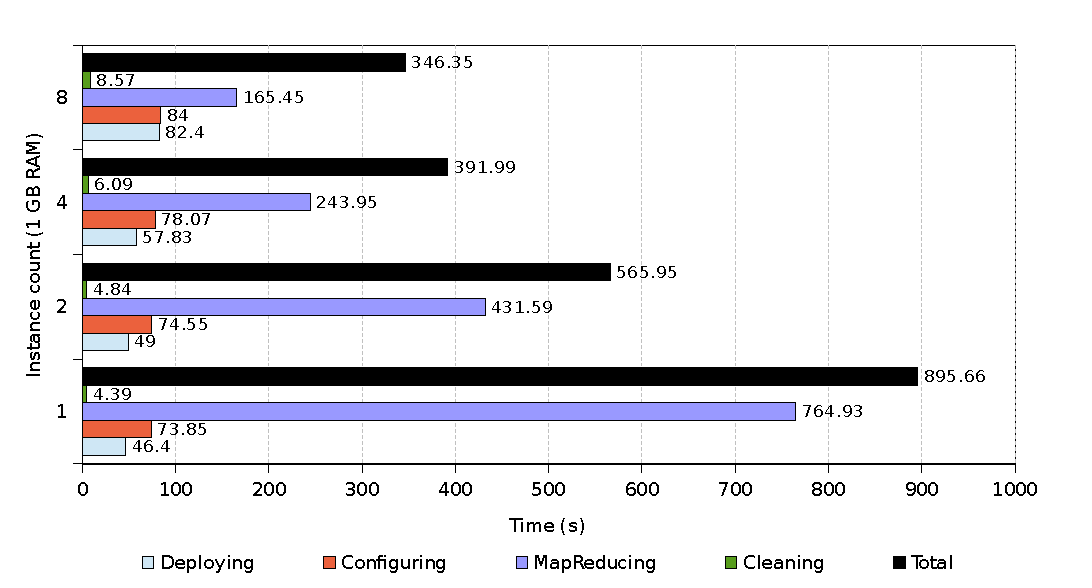
\includegraphics[width=0.98\textwidth]{imagenes/039.pdf}
\caption{Scaling out}
\label{fig:eschorizontal}
\end{center}
\end{figure}

\noindent Figure \ref{fig:eschorizontal} shows the evolution of the different timings as the instance count increases from one to eight. It may be observed that deployment, configuring and cleaning time raise with the number of instances deployed, meanwhile processing time is reduced. I.e, the time required for a virtual cluster to deploy, configure and delete every instance depends only on its size --- as it could have been hypothesized. On the other hand, MapReducing time --- and thus total time --- is also bound to input size. Figure \ref{fig:escvertical} presents the tendency of the five timings as the cluster is scaled in from 1 GB of VCPU and RAM to 4 each.

\begin{figure}[tbp]
\begin{center}
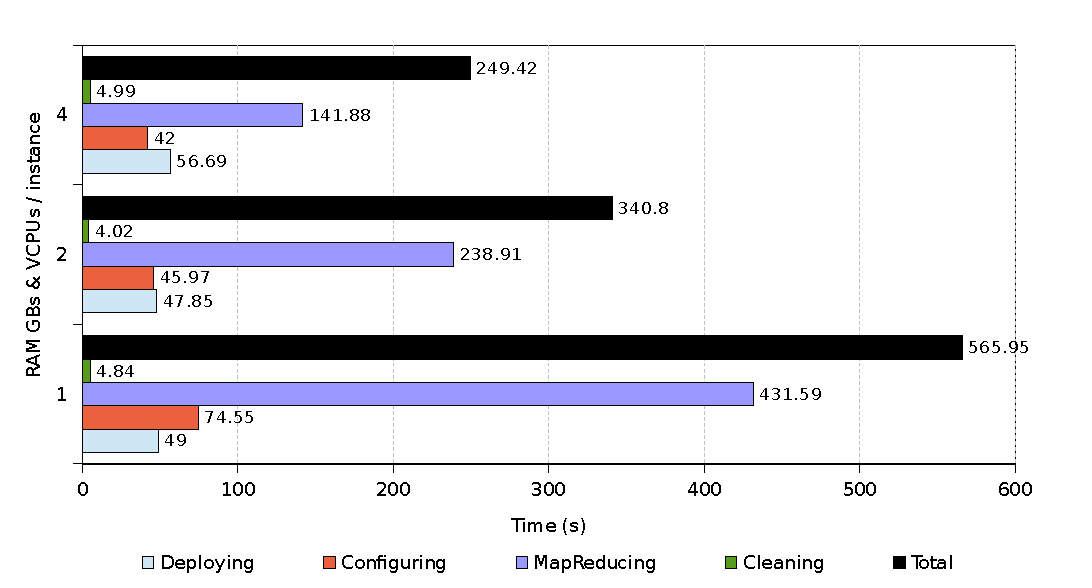
\includegraphics[width=0.98\textwidth]{imagenes/041.pdf}
\caption{Scaling in}
\label{fig:escvertical}
\end{center}
\end{figure}



A la vista de esta figura, tal vez lo m\'as llamativo sean los tiempos de des\-plie\-gue y borrado, pudiendo considerarse pr\'acticamente constantes a pesar de aumentar la capacidad de c\'alculo de las instancias. Dicho de otro modo, la dificultad que supone desplegar o borrar un cl\'uster virtual en nuestro entorno depende exclusivamente del n\'umero de instancias o nodos virtuales ---conclusi\'on que ya hab\'iamos alcanzado previamente. Precisamente, hab\'iamos observado c\'omo la complejidad de configuraci\'on crec\'ia proporcionalmente con el tama\~no del cl\'uster. En este caso sucede lo contrario: al estar mejorando las caracter\'isticas t\'ecnicas de las dos instancias, los tiempos de configuraci\'on de Hadoop se ven l\'ogicamente reducidos. Es decir, la conclusi\'on revisada dicta que el tiempo de configuraci\'on var\'ia de forma directa con el n\'umero de instancias y de forma inversa con las capacidades operativas de las mismas. \newline

Los resultados contenidos en estas gr\'aficas demuestran que nuestra soluci\'on se comporta de modo m\'as eficaz cuando se mejora la capacidad de c\'omputo de las instancias ---escalabilidad vertical--- en vez de aumentar el tama\~no del cl\'uster virtual soporte ---escalabilidad horizontal. Este hecho se observa con claridad en las figuras \ref{fig:eschorizontal} y \ref{fig:escvertical} al comparar los casos extremos de prueba: ocho instancias de 1 GB de RAM frente a 4 GB de RAM y VCPUs por ins\-tan\-cia, respectivamente. Ambos casos distribuyen sendos clusters virtuales con las mismas caracter\'isticas de 8 VCPUs y 8 GB de RAM sobre nuestros nodos de prueba. Sin embargo, el tiempo de ejecuci\'on total es casi un \texttt{28\%} menor al mejorar las dos instancias (figura \ref{fig:escvertical}); esperable, en cierta medida, al ahorrar la sobrecarga de comunicaci\'on por la red. \newline

\begin{figure}[tbp]
\begin{center}
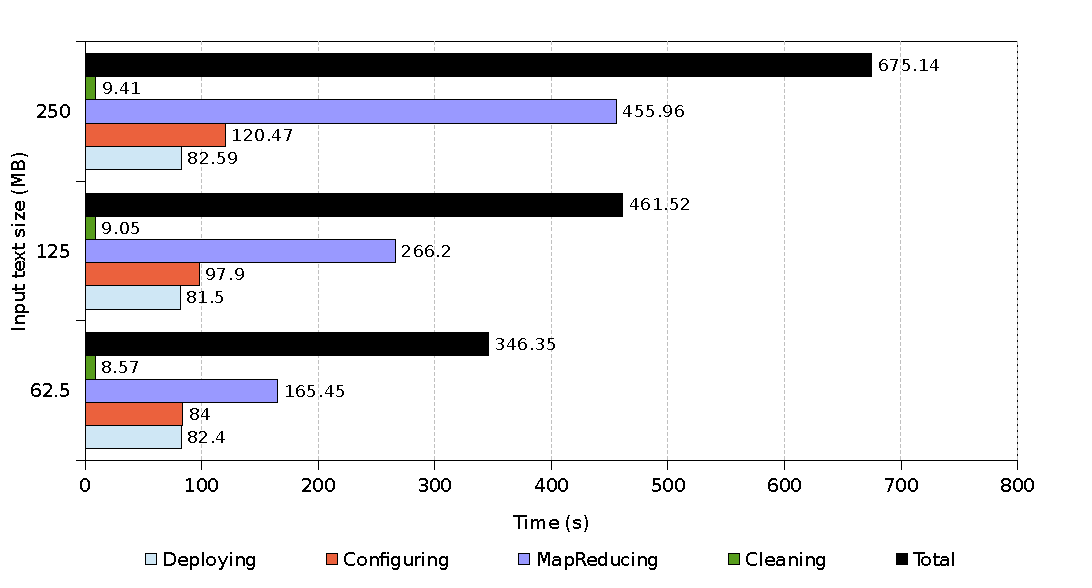
\includegraphics[width=0.98\textwidth]{imagenes/042.pdf}
\caption{Tama\~no de entrada frente a tiempo de ejecuci\'on}
\label{fig:evotemporal}
\end{center}
\end{figure}

La figura \ref{fig:evotemporal} muestra la evoluci\'on de los tiempos de ejecuci\'on al incrementar la magnitud de los datos a procesar. Como era de esperar, la duraci\'on de la etapa MapReduce y la duraci\'on total crecen en relaci\'on directa con el tama\~no de entrada, pero en menor medida. Los tiempos de despliegue y bo\-rra\-do se mantienen pr\'acticamente constantes en cada caso, mientras que el tiempo de configuraci\'on crece ligeramente, al englobar la descompresi\'on y posterior distribuci\'on de los ficheros de entrada sobre el cl\'uster Hadoop.
